% =====================================================================
%  Four in a Row AI — Project Report
%  Build:  pdflatex report.tex  (run twice for the table of contents)
% =====================================================================
\documentclass[11pt,a4paper]{article}

% ---------- Fill these in before submission (leave empty to hide) ----------
\newcommand{\institution}{}          % e.g. Department of Computer Science, XYZ University
\newcommand{\instructor}{}           % e.g. Prof. A. B. Name
\newcommand{\coursename}{Artificial Intelligence Laboratory}
\newcommand{\reportdate}{November 2026}
\newcommand{\repourl}{https://github.com/manishsn7340/Four-in-a-row-2}
% ---------------------------------------------------------------------------

\usepackage[T1]{fontenc}
\usepackage[utf8]{inputenc}
\usepackage[lining]{libertine}
\usepackage[libertine]{newtxmath}
\usepackage[scaled=0.92,varqu]{zi4}
\usepackage{microtype}
\usepackage[a4paper,margin=2.4cm,headheight=14pt]{geometry}
\usepackage[table]{xcolor}
\usepackage{graphicx,booktabs,tabularx,array,multirow,amsmath}
\usepackage{enumitem}
\usepackage{titlesec,fancyhdr}
\usepackage{caption,subcaption}
\usepackage{algorithm}
\usepackage[noend]{algpseudocode}
\usepackage{tikz}
\usetikzlibrary{positioning,arrows.meta,calc,fit,shapes.geometric,backgrounds}
\usepackage{pgfplots}
\pgfplotsset{compat=1.18}
\usepgfplotslibrary{groupplots}
\usepackage[most]{tcolorbox}
\usepackage{siunitx}
\usepackage[hidelinks]{hyperref}
\usepackage[capitalise,noabbrev]{cleveref}

% ---------- Palette (matches the presentation and the app) ----------
\definecolor{plum}{HTML}{2E1065}
\definecolor{violet}{HTML}{7C3AED}
\definecolor{lavender}{HTML}{F3E8FF}
\definecolor{lavmid}{HTML}{DDD0F7}
\definecolor{peach}{HTML}{FFF7ED}
\definecolor{coral}{RGB}{232,86,76}
\definecolor{gold}{RGB}{244,192,62}
\definecolor{boardblue}{HTML}{2F5BD3}
\definecolor{ink}{HTML}{1F1A2E}
\definecolor{muted}{HTML}{6B6480}
\definecolor{good}{HTML}{2E9E6B}
\color{ink}

\hypersetup{colorlinks=true,linkcolor=plum,urlcolor=violet,citecolor=violet,
  pdftitle={Four in a Row AI: Adversarial Search and Monte Carlo Tree Search in an Explainable Strategy Coach},
  pdfauthor={Satyam Singh, Shivam Chaurasia, Manish Shroyan, Mitu Kumar}}

% ---------- Headings ----------
\titleformat{\section}{\sffamily\Large\bfseries\color{plum}}{\color{violet}\thesection}{0.8em}{}
\titleformat{\subsection}{\sffamily\large\bfseries\color{plum}}{\color{violet}\thesubsection}{0.7em}{}
\titleformat{\subsubsection}{\sffamily\normalsize\bfseries\color{plum}}{\thesubsubsection}{0.6em}{}
\titlespacing*{\section}{0pt}{2.2ex plus .5ex}{1.1ex}
\titlespacing*{\subsection}{0pt}{1.8ex plus .4ex}{0.8ex}

\pagestyle{fancy}
\fancyhf{}
\fancyhead[L]{\sffamily\small\color{muted}Four in a Row AI}
\fancyhead[R]{\sffamily\small\color{muted}\nouppercase{\leftmark}}
\fancyfoot[C]{\sffamily\small\color{muted}\thepage}
\renewcommand{\headrulewidth}{0.4pt}
\renewcommand{\headrule}{\hbox to\headwidth{\color{lavmid}\leaders\hrule height \headrulewidth\hfill}}
\renewcommand{\sectionmark}[1]{\markboth{#1}{}}

\captionsetup{font=small,labelfont={bf,color=plum,sf},format=plain,margin=8pt}
\setlist{itemsep=2pt,topsep=4pt}
\setlength{\parskip}{4pt}
\setlength{\parindent}{0pt}
\renewcommand{\arraystretch}{1.18}
\sisetup{group-separator={,},group-minimum-digits=4}

% ---------- Boxes ----------
\newtcolorbox{keybox}[1][]{enhanced,colback=lavender,colframe=violet,boxrule=0pt,
  leftrule=3pt,arc=2pt,left=10pt,right=10pt,top=6pt,bottom=6pt,fonttitle=\sffamily\bfseries,
  coltitle=plum,attach title to upper={\ \ },#1}
\newtcolorbox{statbox}{enhanced,colback=white,colframe=lavmid,boxrule=0.6pt,arc=4pt,
  left=4pt,right=4pt,top=6pt,bottom=6pt,halign=center,valign=center}
\newcommand{\stat}[2]{\begin{statbox}{\sffamily\bfseries\LARGE\color{violet}#1}\\[1pt]{\sffamily\footnotesize\color{muted}#2}\end{statbox}}
\newcommand{\code}[1]{\texttt{\small #1}}
\newcolumntype{Y}{>{\raggedright\arraybackslash}X}
\newcolumntype{C}{>{\centering\arraybackslash}X}

% Small Connect Four board: \cfboard{scale}{list of col/row/player}
\newcommand{\cfboard}[2]{%
  \begin{tikzpicture}[scale=#1]
    \fill[boardblue,rounded corners=3pt] (-0.1,-0.1) rectangle (7.1,6.1);
    \foreach \c in {0,...,6}{\foreach \r in {0,...,5}{\fill[white] (\c+0.5,\r+0.5) circle (0.38);}}
    \foreach \c/\r/\p in {#2}{%
      \ifnum\p=1 \fill[coral] (\c+0.5,\r+0.5) circle (0.38);\else\fill[gold] (\c+0.5,\r+0.5) circle (0.38);\fi}
  \end{tikzpicture}}

% Algorithm style
\algrenewcommand\algorithmicrequire{\textbf{Input:}}
\algrenewcommand\algorithmicensure{\textbf{Output:}}
\makeatletter\renewcommand{\ALG@name}{Algorithm}\makeatother
\floatname{algorithm}{\sffamily\color{plum}Algorithm}

\begin{document}

% =====================================================================
%  TITLE PAGE
% =====================================================================
\begin{titlepage}
\thispagestyle{empty}
\begin{tikzpicture}[remember picture,overlay]
  \fill[peach] (current page.south west) rectangle (current page.north east);
  \fill[lavender,opacity=0.9] ($(current page.north east)+(-9,0)$) rectangle (current page.south east);
  \fill[plum] (current page.north west) rectangle ($(current page.north east)+(0,-1.1)$);
  \node[anchor=west,text=white,font=\sffamily\small] at ($(current page.north west)+(2.4,-0.55)$)
     {\coursename\ifx\institution\empty\else\ \ \textbullet\ \ \institution\fi};
  \node[anchor=south east,opacity=0.95] at ($(current page.south east)+(-1.4,2.2)$)
     {\cfboard{0.62}{3/0/1,3/1/2,2/0/2,4/0/1,3/2/1,2/1/2,4/1/1,2/2/2,1/0/1,5/0/2,4/2/1,1/1/2,4/3/2,5/1/1}};
\end{tikzpicture}

\vspace*{2.4cm}
{\sffamily\small\bfseries\color{violet}PROJECT REPORT \textbullet\ GROUP ASSIGNMENT}\par\vspace{0.5cm}
{\fontsize{40}{44}\selectfont\bfseries\color{plum}Four in a Row AI}\par\vspace{0.4cm}
{\Large\itshape\color{ink} Adversarial Search and Monte Carlo Tree Search\\[2pt] in an Explainable Strategy Coach}\par
\vspace{0.9cm}
{\color{violet}\rule{6cm}{1.6pt}}\par\vspace{0.9cm}

\begin{minipage}[t]{0.55\textwidth}
{\sffamily\small\bfseries\color{muted}SUBMITTED BY}\par\vspace{4pt}
\renewcommand{\arraystretch}{1.35}
\begin{tabular}{@{}l}
\large Satyam Singh\\
\large Shivam Chaurasia\\
\large Manish Shroyan\\
\large Mitu Kumar\\
\end{tabular}
\ifx\instructor\empty\else
\par\vspace{0.6cm}{\sffamily\small\bfseries\color{muted}SUBMITTED TO}\par\vspace{4pt}{\large\instructor}
\fi
\par\vspace{0.8cm}
{\sffamily\small\bfseries\color{muted}SOURCE CODE}\par\vspace{4pt}
\href{\repourl}{\small\texttt{github.com/manishsn7340/Four-in-a-row-2}}
\par\vspace{0.8cm}
{\sffamily\small\bfseries\color{muted}DATE}\par\vspace{4pt}\reportdate
\end{minipage}
\end{titlepage}

% =====================================================================
%  ABSTRACT + CONTENTS
% =====================================================================
\pagenumbering{roman}
\thispagestyle{plain}
\section*{Abstract}
\addcontentsline{toc}{section}{Abstract}

This report presents \emph{Four in a Row AI}, a Connect Four system that plays strong moves and also shows its reasoning. The project implements and compares two families of game-playing algorithms behind one common interface. The first is depth-limited adversarial search: Minimax, Alpha-Beta pruning, centre-first move ordering, time-bounded iterative deepening and a Zobrist-hashed transposition table. The second is Monte Carlo Tree Search with the UCB1 selection rule. A threat-based evaluation function scores all 69 four-cell lines of the board, and a lightweight opponent model predicts the human player's next move and describes their playing style. Everything runs inside a Pygame application that works as a \emph{strategy coach}: a live ``who is ahead'' bar, per-column hint scores with plain-language reasons, engine statistics, tactical puzzles and AI-versus-AI matches.

Four reproducible experiments measure the work. An ablation study shows that the Alpha-Beta optimisations together cut the positions searched per move by \textbf{67\%} (233 to 78) at the same depth, with no change in playing strength. A round-robin tournament confirms that deeper search wins (the depth-7 agent won 46 of its 60 games). A depth study measures an effective branching factor of about \textbf{4.7}, against 7 for an unpruned tree. A 180-game weight study shows that, at a fixed depth, the tested evaluation weight sets do not differ significantly. Correctness is backed by \textbf{209 automated tests}, including invariant checks that Alpha-Beta always agrees with Minimax and that every search leaves the board exactly as it found it.

\vspace{0.4cm}
\noindent\begin{minipage}{\textwidth}
\begin{tabularx}{\textwidth}{@{}CCCC@{}}
\stat{5}{AI agents} & \stat{$-$67\%}{search work at equal depth} & \stat{209}{automated tests} & \stat{4}{reproducible studies}
\end{tabularx}
\end{minipage}

\vspace{0.3cm}
\textbf{Keywords:} Connect Four, adversarial search, Minimax, Alpha-Beta pruning, iterative deepening, transposition table, Zobrist hashing, Monte Carlo Tree Search, UCT, heuristic evaluation, explainable AI.

\clearpage
{\hypersetup{linkcolor=ink}\tableofcontents}
\clearpage
\pagenumbering{arabic}

% =====================================================================
\section{Introduction}
% =====================================================================

Board games have been a benchmark for artificial intelligence since Shannon's 1950 paper on computer chess~\cite{shannon1950}. They have clear rules, a well-defined winner and a search space too large to explore completely, so they force a program to make good decisions under limited computation. That is exactly the problem adversarial search was designed for~\cite{aima}.

\emph{Connect Four} (also called Four in a Row) is played on a vertical grid of 6 rows and 7 columns. Two players take turns dropping a disc into a column, and the disc falls to the lowest empty cell. The first player to line up four of their own discs horizontally, vertically or diagonally wins, and a full board with no line of four is a draw. The rules fit in one paragraph, but the game has about $4.5\times10^{12}$ reachable positions~\cite{edelkamp2008}, far too many to search during play.

Our assignment asked for a Python Connect Four game with an AI opponent that uses Minimax with Alpha-Beta pruning to \emph{evaluate possible moves, predict the player's strategy and choose optimal plays}. We treated that brief as the minimum. The result is a complete, tested system with five interchangeable agents, two different AI paradigms, four measured experiments and an application that explains what the AI is thinking.

\paragraph{Report structure.} \Cref{sec:problem,sec:objectives} define the problem and objectives. \Cref{sec:novelty} sets out what is new in this project and what we contribute. \Cref{sec:background} reviews the background algorithms. \Cref{sec:design,sec:method} describe the architecture and every agent in detail. \Cref{sec:app} presents the application, \cref{sec:setup,sec:results} the experiments and their results, and \cref{sec:testing} the testing strategy. The report closes with limitations, future work and conclusions.

% =====================================================================
\section{Problem Statement}\label{sec:problem}
% =====================================================================

\begin{keybox}[title=Problem]
Design and build a computer opponent for Connect Four that chooses strong moves within a time budget a human will accept (under about two seconds). It must anticipate the opponent's replies and make its reasoning visible to the person playing against it. Then measure, rather than assume, how much each algorithmic technique contributes.
\end{keybox}

\subsection{Formal definition}
We model Connect Four as a deterministic, two-player, zero-sum game of perfect information~\cite{aima}:

\begin{itemize}
  \item \textbf{States} $s$: an assignment of $\{\text{empty},\text{P1},\text{P2}\}$ to the $6\times7$ cells that respects gravity (no disc floats above an empty cell).
  \item \textbf{Player} $\textsc{To-Move}(s)$: P1 if an even number of discs has been played, otherwise P2. P1 always moves first.
  \item \textbf{Actions} $\textsc{Actions}(s)$: the columns whose top cell is empty, so at most 7.
  \item \textbf{Transition} $\textsc{Result}(s,a)$: the current player's disc lands in the lowest empty cell of column $a$.
  \item \textbf{Terminal test}: a player has four in a row, or the board is full (42 discs).
  \item \textbf{Utility}: $+1$ for a win, $-1$ for a loss and $0$ for a draw, from the root player's point of view.
\end{itemize}

\subsection{Why the problem is hard}
With up to 7 legal moves per turn and games lasting up to 42 moves, a full game tree has on the order of $7^{d}$ nodes to depth $d$: about 117{,}649 at depth 6 and over 40 million at depth 9. Connect Four was solved in 1988, independently by James D.\ Allen and by Victor Allis~\cite{allis1988}: the first player wins with perfect play by starting in the centre column. That proof relies on extensive expert knowledge and precomputed databases, though. A game-playing program must instead decide in real time, from an incomplete look-ahead, which means it needs (i) an efficient search that skips provably irrelevant branches and (ii) a heuristic evaluation for positions where the search has to stop.

\subsection{Scope}
\textbf{In scope:} standard $6\times7$ Connect Four; human-vs-AI, human-vs-human and AI-vs-AI play; CPU-only Python implementation using only the standard library, \code{pygame}, \code{numpy}, \code{matplotlib}, \code{pandas} and \code{pytest}.\\
\textbf{Out of scope:} perfect play from a solved database, other board sizes, networked play and machine-learned evaluation.

% =====================================================================
\section{Objectives}\label{sec:objectives}
% =====================================================================

\begin{enumerate}[label=\textbf{O\arabic*.},leftmargin=2.2em]
  \item \textbf{Correct game engine.} Implement the board, gravity, legal moves, undo and an efficient win check, verified by tests.
  \item \textbf{Adversarial search.} Implement Minimax and Alpha-Beta pruning, and prove that Alpha-Beta always returns the same decision as Minimax at equal depth.
  \item \textbf{Search optimisation.} Add move ordering, iterative deepening with a hard time limit, and a transposition table with Zobrist hashing, each switchable on or off.
  \item \textbf{Heuristic evaluation.} Design a threat-aware evaluation function that is symmetric between players and has tunable weights.
  \item \textbf{Alternative paradigm.} Implement Monte Carlo Tree Search (UCT) as a simulation-based contrast to evaluation-based search.
  \item \textbf{Player modelling.} Predict the human player's next move and describe their playing style.
  \item \textbf{Explainable application.} Build a responsive GUI that shows the AI's reasoning: evaluation, hints, search statistics and puzzles.
  \item \textbf{Empirical evaluation.} Measure every technique with reproducible experiments (fixed seeds, fair openings) and report the results honestly.
\end{enumerate}

% =====================================================================
\section{Novelty and Contributions}\label{sec:novelty}
% =====================================================================

Minimax and Alpha-Beta for Connect Four are textbook material. Our project does not claim new search algorithms. Its novelty lies in \emph{how} the system is built, evaluated and presented.

\subsection{Novelty}
\begin{enumerate}[label=\textbf{N\arabic*.},leftmargin=2.2em]
  \item \textbf{An AI that explains itself.} Most Connect Four programs only play. Ours works as a coach: it shows who is ahead, scores every column for a hint, gives a one-line reason in plain language, predicts the player's next move and streams live search statistics (positions searched, branches pruned, depth reached).
  \item \textbf{Two AI paradigms behind one interface.} Every agent, from a random player to MCTS, implements the same \code{choose\_move(board)\,$\to$\,column} contract, so evaluation-based search and simulation-based search can face each other directly and fairly.
  \item \textbf{Each optimisation measured in isolation.} An ablation study turns on one technique at a time, so the contribution of pruning, ordering, iterative deepening and the transposition table is a measured number, not a claim.
  \item \textbf{A fair protocol for deterministic agents.} Search agents always play the same move in the same position, so naive repeated matches only replay the same two games. We found this problem and fixed it with seeded random openings played once from each side (\cref{sec:setup}).
  \item \textbf{Correctness as an executable property.} Key invariants are automated tests: Alpha-Beta equals Minimax, the transposition table never changes a result, the evaluation is symmetric, and every agent restores the board exactly.
\end{enumerate}

\subsection{Contributions}
\begin{itemize}
  \item A layered, tested Connect Four engine with incremental Zobrist hashing (\cref{sec:design}).
  \item Five interchangeable agents (Random, Greedy, Minimax, configurable Alpha-Beta and MCTS) plus a player-prediction module (\cref{sec:method}).
  \item A 69-window threat-based evaluation function with a single weights dictionary (\cref{sec:eval}).
  \item A Pygame strategy-coach application with four AI personas, hints, puzzles and themes (\cref{sec:app}).
  \item Four reproducible experiments with CSV outputs and plots (\cref{sec:results}).
  \item A suite of 209 automated tests (\cref{sec:testing}) and a report generator that refuses to publish results unless every test passes.
\end{itemize}

\subsection{Source code}
The full source code, experiment scripts, results and this project's tests are publicly available at:
\begin{center}
\begin{tcolorbox}[enhanced,colback=white,colframe=violet,boxrule=0.8pt,arc=3pt,width=0.8\textwidth,halign=center]
\href{\repourl}{\large\texttt{\repourl}}
\end{tcolorbox}
\end{center}

% =====================================================================
\section{Background}\label{sec:background}
% =====================================================================

\paragraph{Minimax.} For two-player zero-sum games, Minimax assumes both players play optimally. At positions where the AI moves it takes the maximum value over the children, and at positions where the opponent moves it takes the minimum~\cite{aima}. Search stops at a fixed depth, where a heuristic \emph{evaluation function} estimates the value~\cite{shannon1950}. With branching factor $b$ and depth $d$, Minimax visits $O(b^d)$ nodes.

\paragraph{Alpha-Beta pruning.} Alpha-Beta keeps two bounds while it searches: $\alpha$, the best value the maximiser can already guarantee, and $\beta$, the best the minimiser can guarantee. Once $\alpha \ge \beta$, the remaining children of a node cannot affect the decision and are skipped. The result is identical to Minimax. With perfect move ordering the node count drops to about $O(b^{d/2})$~\cite{knuth1975}, so in the same time the search can go roughly twice as deep.

\paragraph{Iterative deepening and transposition tables.} Iterative deepening searches to depth $1, 2, 3, \dots$ and returns the result of the last depth it completed, which turns a fixed-depth search into an \emph{anytime} algorithm~\cite{korf1985}. Different move orders often reach the same position (a \emph{transposition}). A transposition table caches results keyed by a position hash. Zobrist hashing~\cite{zobrist1970} computes that hash incrementally with one XOR per move.

\paragraph{Monte Carlo Tree Search.} MCTS builds a search tree from random simulations instead of an evaluation function~\cite{browne2012}. Each iteration has four phases: \emph{selection}, \emph{expansion}, \emph{simulation} and \emph{backpropagation}. The UCT variant~\cite{kocsis2006} selects children with the UCB1 bandit formula~\cite{auer2002}, which balances exploiting moves that won often against exploring moves that have been tried rarely.

\clearpage
% =====================================================================
\section{System Design}\label{sec:design}
% =====================================================================

\subsection{Layered architecture}
The project was built in ten layers. Each layer depends only on the layers before it and arrived with its own tests (\cref{fig:arch}). This let us verify each piece before building on it.

\begin{figure}[ht]
\centering
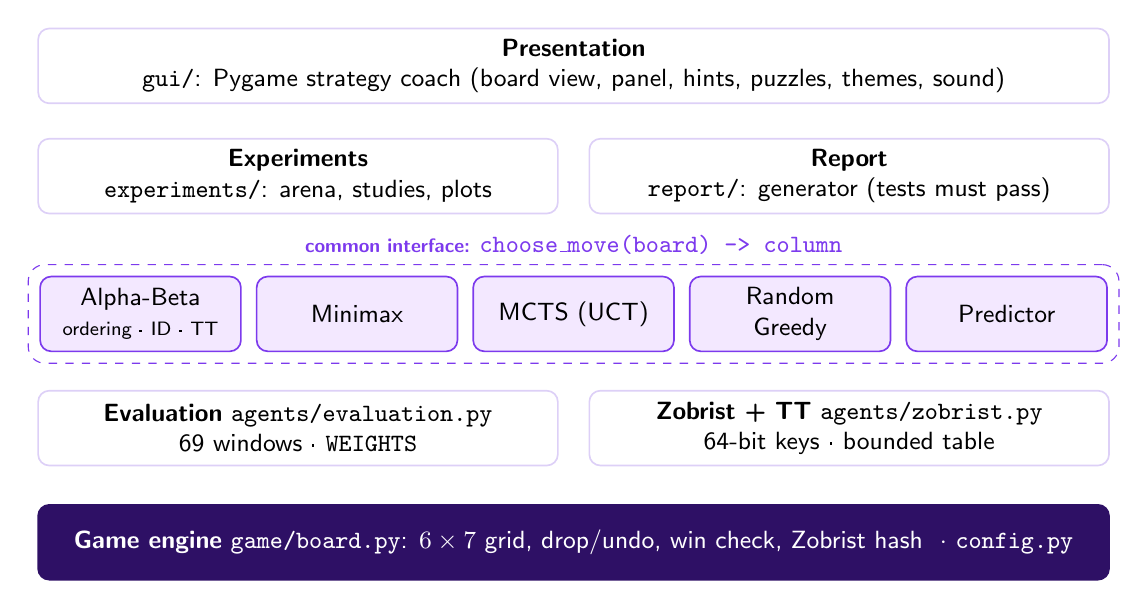
\begin{tikzpicture}[
  layer/.style={draw=lavmid,fill=white,rounded corners=4pt,minimum height=0.95cm,font=\sffamily\small,align=center,line width=0.6pt},
  hl/.style={layer,fill=lavender,draw=violet},
  lbl/.style={font=\sffamily\scriptsize\bfseries,text=muted,anchor=east}]
  % rows
  \node[layer,minimum width=13.6cm] (gui) at (0,4.75) {\textbf{Presentation} \\ \code{gui/}: Pygame strategy coach (board view, panel, hints, puzzles, themes, sound)};
  \node[layer,minimum width=6.6cm] (exp) at (-3.5,3.35) {\textbf{Experiments} \\ \code{experiments/}: arena, studies, plots};
  \node[layer,minimum width=6.6cm] (rep) at (3.5,3.35) {\textbf{Report} \\ \code{report/}: generator (tests must pass)};
  \node[hl,minimum width=2.55cm] (ab) at (-5.5,1.6) {Alpha-Beta\\\scriptsize ordering · ID · TT};
  \node[hl,minimum width=2.55cm] (mm) at (-2.75,1.6) {Minimax};
  \node[hl,minimum width=2.55cm] (mc) at (0,1.6) {MCTS (UCT)};
  \node[hl,minimum width=2.55cm] (sm) at (2.75,1.6) {Random\\Greedy};
  \node[hl,minimum width=2.55cm] (pr) at (5.5,1.6) {Predictor};
  \node[layer,minimum width=6.6cm] (ev) at (-3.5,0.15) {\textbf{Evaluation} \code{agents/evaluation.py}\\69 windows · \code{WEIGHTS}};
  \node[layer,minimum width=6.6cm] (zb) at (3.5,0.15) {\textbf{Zobrist + TT} \code{agents/zobrist.py}\\64-bit keys · bounded table};
  \node[layer,minimum width=13.6cm,fill=plum,text=white,draw=plum] (bd) at (0,-1.3) {\textbf{Game engine} \code{game/board.py}: $6\times7$ grid, drop/undo, win check, Zobrist hash \ $\cdot$\ \code{config.py}};
  \node[fit=(ab)(pr),draw=violet,dashed,rounded corners=6pt,inner sep=4pt,
        label={[font=\sffamily\scriptsize\bfseries,text=violet]above:{common interface: \code{choose\_move(board) -> column}}}] {};
\end{tikzpicture}
\caption{Layered architecture. Arrows are implicit: every layer uses only the layers below it. All agents (highlighted) share one interface, so the GUI and the experiments can use any of them.}
\label{fig:arch}
\end{figure}

\subsection{Board representation}
The board (\code{game/board.py}) stores \code{grid[row][col]} with row~0 at the bottom, plus a \code{move\_history} list. The player to move is derived from the length of the history, so it can never go out of sync. The key design decisions are:

\begin{itemize}
  \item \textbf{In-place \code{drop}/\code{undo}.} Search explores millions of positions, and copying the board at every node would dominate the run time. Instead every search makes a move, recurses and undoes it. A project rule, enforced by tests, requires each agent to return the board \emph{exactly} as it received it.
  \item \textbf{Local win check.} A new win can only pass through the disc just played, so \code{winner()} checks only the four lines through the last move instead of scanning the board. A test over 1{,}000 seeded random games confirmed that it always agrees with a full-board scan.
  \item \textbf{Incremental hash.} Every \code{drop} and \code{undo} XORs one Zobrist key into \code{board.hash}, so a position's fingerprint is always available in $O(1)$ (\cref{sec:tt}).
  \item \textbf{Validated input.} Boards can be saved to and loaded from text. Loading rejects impossible positions such as floating discs.
\end{itemize}

\subsection{Engineering principles}
All constants live in \code{config.py} (board size, $\textsc{Win}=10^6$, move order, table size, seeds, UCB constant). All randomness goes through an explicit \code{random.Random(seed)}, so every game and experiment can be reproduced exactly. There is no global mutable state, and no dependency is used beyond the five libraries listed in \cref{sec:problem}.

% =====================================================================
\section{Methodology: The Agents}\label{sec:method}
% =====================================================================

\Cref{tab:agents} summarises the agents. Every one of them fills in a \code{SearchStats} record (positions searched, cut-offs, table hits, depth reached, simulations, time, per-column scores), which the GUI displays and the experiments log.

\begin{table}[ht]
\centering\small
\caption{The agent family. All agents implement \code{choose\_move(board) -> column}.}
\label{tab:agents}
\begin{tabularx}{\textwidth}{@{}l l Y@{}}
\toprule
\textbf{Agent} & \textbf{File} & \textbf{How it decides} \\
\midrule
Random   & \code{agents/simple.py}    & Seeded uniform choice among legal columns (baseline). \\
Greedy   & \code{agents/simple.py}    & Win if possible, else block an immediate loss, else play nearest the centre. \\
Minimax  & \code{agents/minimax.py}   & Full fixed-depth game-tree search with the evaluation at the leaves. \\
Alpha-Beta & \code{agents/alphabeta.py} & Minimax with pruning, plus optional move ordering, iterative deepening and a transposition table. \\
MCTS     & \code{agents/mcts.py}      & UCT tree search guided by random play-outs; no evaluation function. \\
\midrule
Predictor & \code{agents/predictor.py} & Not a player: predicts the human's next move and describes their style. \\
\bottomrule
\end{tabularx}
\end{table}

% ---------------------------------------------------------------
\subsection{Evaluation function}\label{sec:eval}
% ---------------------------------------------------------------
When a search stops before the game ends, the position is scored by \code{evaluate(board, player, weights)} in \code{agents/evaluation.py}.

\paragraph{Windows.} Every way to make four in a row is a \emph{window} of four cells. At import time the program lists all of them once: 24 horizontal, 21 vertical and 24 diagonal, \textbf{69 windows} in total. A window that contains a disc of both players can never be completed, so it is ignored.

\paragraph{Scoring one side.} For player $p$, with $w$ the weights in \cref{tab:weights}:
\begin{equation}
S(p) \;=\; w_{\text{centre}}\,C_p \;+\; w_{\text{two}}\,|W_2(p)| \;+\! \sum_{t\,\in\, W_3(p)} \!\big(w_{\text{three}} + w_{\text{playable}}\,[\,t \text{ playable}\,]\big) \;+\; w_{\text{double}}\,[\,|T_p|\ge 2\,]
\end{equation}
Here $C_p$ is the number of $p$'s discs in the centre column, $W_2(p)$ and $W_3(p)$ are the open windows holding exactly two and three of $p$'s discs, a three's gap is \emph{playable} when the empty cell is exactly where the next disc in that column would land, and $T_p$ is the set of columns where $p$ could complete four immediately. Two or more such columns form a \emph{double threat}, which the opponent cannot block with one move.

\paragraph{Final score.} The evaluation is the difference between the two sides, and terminal positions get exact values:
\begin{equation}
\text{eval}(s,p) = \begin{cases} +10^6 & p \text{ has won}\\ -10^6 & \text{the opponent has won}\\ 0 & \text{draw}\\ S(p) - S(\bar p) & \text{otherwise.}\end{cases}
\end{equation}
Because the same rules score both sides, the function is \emph{symmetric}: $\text{eval}(s,1) = -\text{eval}(s,2)$. A test checks this on 100 seeded positions. In a 40-game match at depth~4, the full evaluation beat a centre-only baseline (\code{BASIC\_WEIGHTS}) by 26 wins to 11, with 3 draws.

\begin{table}[ht]
\centering\small
\caption{Default evaluation weights (\code{WEIGHTS}). Opponent terms come from the symmetric difference, so the keys \code{opp\_two} and \code{opp\_three} exist in the dictionary but are not read.}
\label{tab:weights}
\begin{tabular}{@{}lcl@{}}
\toprule
\textbf{Feature} & \textbf{Weight} & \textbf{Meaning} \\
\midrule
\code{center} & 3 & per disc in the centre column (it lies on the most windows) \\
\code{two} & 2 & open window with two own discs \\
\code{three} & 5 & open window with three own discs \\
\code{playable\_three} & +8 & bonus when that three can be completed on the next move \\
\code{double\_threat} & 40 & two or more columns that win immediately \\
\bottomrule
\end{tabular}
\end{table}

% ---------------------------------------------------------------
\subsection{Baselines: Random and Greedy}
% ---------------------------------------------------------------
\textbf{Random} picks a legal column with a seeded generator. \textbf{Greedy} looks one move ahead: it takes an immediate win, otherwise blocks the opponent's immediate win, otherwise plays the legal column closest to the centre in the order $3,2,4,1,5,0,6$. They are reference points: any search agent must beat them clearly, and tests check that it does (for example, Minimax at depth~3 wins at least 18 of 20 seeded games against Random).

% ---------------------------------------------------------------
\subsection{Minimax}
% ---------------------------------------------------------------
Minimax (\cref{alg:minimax}) explores every legal move to a fixed depth. Win scores include the remaining depth, $\pm(10^6 + \text{depth})$, so the agent prefers \emph{faster} wins and \emph{slower} losses. Without this, a win in one move and a win in five would look equal, and the agent could delay a win indefinitely.

\begin{algorithm}[ht]
\caption{Depth-limited Minimax (\code{agents/minimax.py})}\label{alg:minimax}
\begin{algorithmic}[1]
\Function{Minimax}{$s$, $d$, \textit{maximising}, \textit{me}}
  \State \textit{nodes} $\gets$ \textit{nodes} $+1$
  \If{a player has won in $s$} \Return $\pm(10^6 + d)$ \Comment{sign: $+$ if \textit{me} won}
  \EndIf
  \If{board full} \Return 0 \EndIf
  \If{$d = 0$} \Return \Call{Evaluate}{$s$, \textit{me}} \EndIf
  \ForAll{column $c$ in \Call{Actions}{$s$}}
     \State \Call{Drop}{$s,c$}; \ $v_c \gets$ \Call{Minimax}{$s$, $d-1$, \textbf{not} \textit{maximising}, \textit{me}}; \ \Call{Undo}{$s$}
  \EndFor
  \State \Return $\max_c v_c$ \textbf{if} \textit{maximising} \textbf{else} $\min_c v_c$
\EndFunction
\end{algorithmic}
\end{algorithm}

% ---------------------------------------------------------------
\subsection{Alpha-Beta pruning}
% ---------------------------------------------------------------
\code{AlphaBetaAgent} carries the window $[\alpha,\beta]$ down the tree (\cref{alg:ab}). When a maximising node finds a value $\ge\beta$, the minimiser above it would never allow this line, so the remaining children are skipped (a \emph{cut-off}), and symmetrically for minimising nodes. Every technique in the following subsections can be switched on or off in the constructor, which is what makes the ablation study possible.

\begin{algorithm}[ht]
\caption{Alpha-Beta with transposition table and move ordering (\code{agents/alphabeta.py})}\label{alg:ab}
\begin{algorithmic}[1]
\Function{AlphaBeta}{$s$, $d$, \textit{max}, $\alpha$, $\beta$}
  \State check the clock every 1{,}024 nodes; raise \textsc{Timeout} past the deadline
  \State $e \gets$ \Call{TT.Get}{\textit{hash}$(s)$}
  \If{$e$ exists \textbf{and} $e.\textit{depth} \ge d$} \Comment{reuse a stored result}
    \If{$e.\textit{flag} = \textsc{Exact}$} \Return $e.\textit{score}$ \EndIf
    \State tighten $\alpha$ (\textsc{Lower}) or $\beta$ (\textsc{Upper}); \textbf{if} $\alpha\ge\beta$ \Return $e.\textit{score}$
  \EndIf
  \If{terminal or $d=0$} \Return exact / heuristic score (as in \cref{alg:minimax}) \EndIf
  \ForAll{$c$ in \Call{Ordered}{$s$, $e.\textit{bestMove}$}} \Comment{TT move first, then centre-out}
    \State \Call{Drop}{$s,c$}; \ $v \gets$ \Call{AlphaBeta}{$s, d-1, \neg\textit{max}, \alpha, \beta$}; \ \Call{Undo}{$s$}
    \State update \textit{best}; \ \textbf{if} \textit{max} \textbf{then} $\alpha\gets\max(\alpha,\textit{best})$ \textbf{else} $\beta\gets\min(\beta,\textit{best})$
    \If{$\alpha \ge \beta$} \textit{cutoffs} $\gets$ \textit{cutoffs}$+1$; \textbf{break} \EndIf
  \EndFor
  \State \Call{TT.Store}{\textit{hash}$(s)$, $d$, \textit{best}, flag from original $[\alpha_0,\beta_0]$, best move}
  \State \Return \textit{best}
\EndFunction
\end{algorithmic}
\end{algorithm}

\paragraph{Correctness guarantee.} Pruning removes only branches that cannot change the decision. A test compares Alpha-Beta and Minimax on 50 seeded positions at depths~1 to 4 and requires the \emph{same move and the same score} every time.

% ---------------------------------------------------------------
\subsection{Move ordering and iterative deepening}
% ---------------------------------------------------------------
\paragraph{Move ordering.} Alpha-Beta prunes most when the best move is searched first. Columns are tried centre-out, $3,2,4,1,5,0,6$, because the centre column lies on the most windows (15 at the edge, 39 one step from the centre and 51 in the centre column itself) and is usually strongest. If the transposition table or the previous iteration knows a best move, that move goes first.

\paragraph{Iterative deepening (ID).} The Grandmaster persona searches depth $1,2,3,\dots$ up to 7 under a 1.5\,s limit. Each iteration starts with the best move of the previous one, which improves ordering. The clock is checked every 1{,}024 positions. When time runs out in the middle of a depth, that unfinished search is discarded and the move from the \emph{last completed} depth is played. The search also stops early once it proves a forced win. The result is an agent that is never late and gets deeper automatically in simple positions.

% ---------------------------------------------------------------
\subsection{Transposition table and Zobrist hashing}\label{sec:tt}
% ---------------------------------------------------------------
\paragraph{Zobrist keys.} At start-up, every (cell, player) pair receives a fixed random 64-bit number from \code{random.Random(42)}: $6\times7\times2 = 84$ keys. A position's hash is the XOR of the keys of all its discs, and the empty board hashes to 0. Because $x \oplus k \oplus k = x$, \code{drop} and \code{undo} each update the hash with a single XOR. Because XOR is commutative, the same position reached by different move orders gets the same hash. The side to move does not need its own key, because in Connect Four the number of discs already determines it.

\paragraph{Table entries and bounds.} The table maps a hash to \code{(depth, score, flag, best\_move)}. A stored score is only exact if the search finished inside its original window $[\alpha_0,\beta_0]$, so each entry also records what kind of bound it is (\cref{tab:bounds}).

\begin{table}[ht]
\centering\small
\caption{Bound flags stored with each transposition-table entry.}\label{tab:bounds}
\begin{tabular}{@{}lll@{}}
\toprule
\textbf{Search ended with} & \textbf{Flag} & \textbf{On a later hit (if stored depth $\ge$ needed)} \\
\midrule
$\alpha_0 < v < \beta_0$ & \textsc{Exact} & return $v$ immediately \\
$v \ge \beta_0$ (cut-off) & \textsc{Lower} & true value $\ge v$: raise $\alpha$ \\
$v \le \alpha_0$ (fail low) & \textsc{Upper} & true value $\le v$: lower $\beta$ \\
\bottomrule
\end{tabular}
\end{table}

\paragraph{Replacement and safety.} A deeper result replaces a shallower one. The table holds at most $10^6$ entries; when it is full, new positions are not stored, which keeps memory bounded. Scores are stored from the root player's point of view, so the table is cleared whenever the agent starts searching for the other colour. Entries are \emph{not} removed when a human undoes moves: they are keyed by position, not by history, so they stay valid. Tests confirm that enabling the table never changes the root score.

% ---------------------------------------------------------------
\subsection{Monte Carlo Tree Search}
% ---------------------------------------------------------------
\code{MCTSAgent} needs no evaluation function. It estimates each move's strength from the outcomes of many simulated games (\cref{fig:mcts}). For each of $N$ simulations (1{,}000 for the Gambler persona, 500 in the tournament):

\begin{enumerate}
  \item \textbf{Selection.} From the root, repeatedly move to the child with the highest UCB1 value while the node is fully expanded:
  \begin{equation}
  \text{UCB1}(i) = \frac{W_i}{N_i} + c\sqrt{\frac{\ln N_{\text{parent}}}{N_i}}, \qquad c = 1.41 \approx \sqrt 2,
  \end{equation}
  where $W_i/N_i$ is the child's win rate (exploitation) and the square-root term favours rarely tried children (exploration). Unvisited children score $\infty$.
  \item \textbf{Expansion.} Add \emph{one} new child for a randomly chosen untried move.
  \item \textbf{Simulation.} Play random legal moves until the game ends. An optional ``light'' play-out takes a win or blocks a loss when it can. Play-out positions are not stored in the tree.
  \item \textbf{Backpropagation.} Walk back to the root, adding 1 visit to every node and crediting the result (win 1, draw 0.5, loss 0) from the point of view of the player who made that node's move.
\end{enumerate}
After the last simulation the agent plays the \emph{most visited} root child, which is more robust than the highest win rate. Two practical details: an immediate win is played without searching, and all randomness comes from a seeded generator, so the same position and seed always give the same move.

\begin{figure}[ht]
\centering
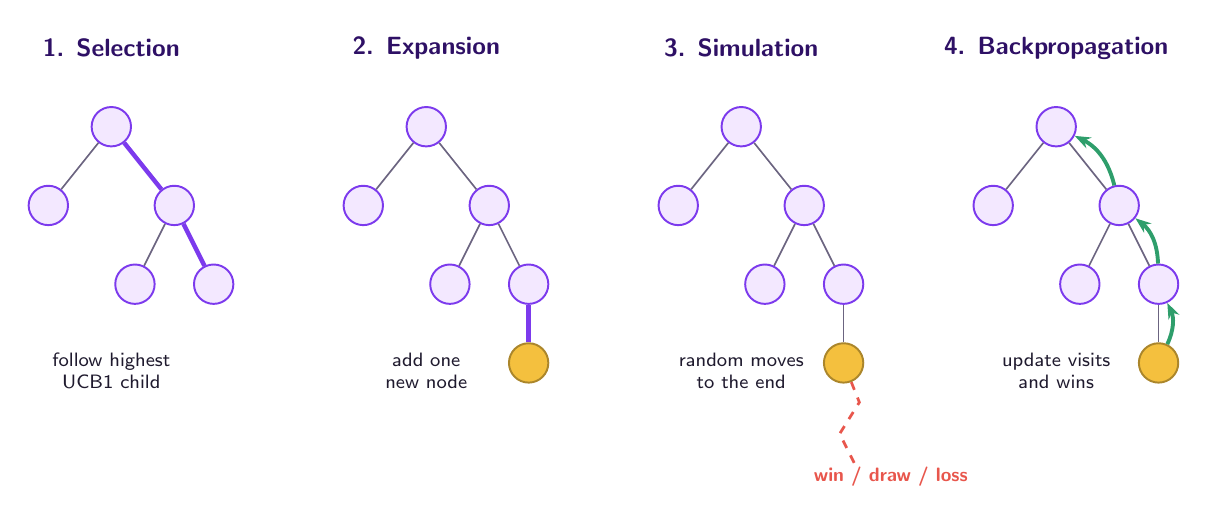
\begin{tikzpicture}[
  n/.style={circle,draw=violet,fill=white,line width=0.7pt,minimum size=5mm,inner sep=0},
  nn/.style={n,fill=lavender},
  newn/.style={n,fill=gold,draw=gold!70!black},
  t/.style={font=\sffamily\scriptsize,align=center,text=ink},
  h/.style={font=\sffamily\small\bfseries,text=plum},
  e/.style={-,draw=muted,line width=0.6pt},
  sel/.style={-,draw=violet,line width=1.6pt}]
  \foreach \X/\name/\label in {0/sel/1. Selection,4/exp/2. Expansion,8/sim/3. Simulation,12/bp/4. Backpropagation}{
    \node[h] at (\X,1.0) {\label};
    \node[nn] (\name r) at (\X,0) {};
    \node[nn] (\name a) at (\X-0.8,-1) {};
    \node[nn] (\name b) at (\X+0.8,-1) {};
    \node[nn] (\name c) at (\X+0.3,-2) {};
    \node[nn] (\name d) at (\X+1.3,-2) {};
    \draw[e] (\name r)--(\name a); \draw[e] (\name r)--(\name b); \draw[e] (\name b)--(\name c); \draw[e] (\name b)--(\name d);
  }
  \draw[sel] (selr)--(selb); \draw[sel] (selb)--(seld);
  \node[t] at (0,-3.1) {follow highest\\UCB1 child};
  \node[newn] (expn) at (5.3,-3) {}; \draw[sel] (expd)--(expn);
  \node[t] at (4,-3.1) {add one\\new node};
  \node[newn] (simn) at (9.3,-3) {};  \draw[e] (simd)--(simn);
  \draw[dashed,draw=coral,line width=1pt,decorate] (simn) -- ++(0.2,-0.5) -- ++(-0.25,-0.4) -- ++(0.2,-0.4);
  \node[font=\sffamily\scriptsize\bfseries,text=coral] at (9.9,-4.45) {win / draw / loss};
  \node[t] at (8,-3.1) {random moves\\to the end};
  \node[newn] (bpn) at (13.3,-3) {}; \draw[e] (bpd)--(bpn);
  \draw[-{Stealth[length=2mm]},draw=good,line width=1.4pt] (bpn) to[bend right=25] (bpd);
  \draw[-{Stealth[length=2mm]},draw=good,line width=1.4pt] (bpd) to[bend right=25] (bpb);
  \draw[-{Stealth[length=2mm]},draw=good,line width=1.4pt] (bpb) to[bend right=25] (bpr);
  \node[t] at (12,-3.1) {update visits\\and wins};
\end{tikzpicture}
\caption{One MCTS iteration. The tree grows by exactly one node (gold) per simulation; repeated thousands of times, visits concentrate on the strongest moves.}
\label{fig:mcts}
\end{figure}

% ---------------------------------------------------------------
\subsection{Predicting the player}
% ---------------------------------------------------------------
The brief asks the AI to \emph{predict the player's strategy}. The search already does this implicitly: at every minimising level, Minimax assumes the opponent picks the reply that is worst for the AI. To make the prediction \emph{visible}, \code{agents/predictor.py} adds an explicit, cheap opponent model that the GUI shows on the human's turn:

\begin{itemize}
  \item \code{predict\_next\_move(board, player)} assumes a one-move-ahead player: (1)~take an immediate win; (2)~otherwise block the opponent's immediate win; (3)~otherwise try each legal column, evaluate the result with \code{WEIGHTS} from the player's side, undo, and predict the highest-scoring column. This costs at most seven evaluations, and the board is restored afterwards.
  \item \code{describe\_style(moves, player)} takes the player's own moves (\code{moves[player-1::2]}) and, after at least three, reports a style: ``favours the centre'' if $\ge$60\% were in the middle three columns, ``left/right side'' if $\ge$40\% were in the two outer columns on one side, otherwise ``mixes up their columns''.
\end{itemize}
The predictor is deliberately separate from the search: it is a coaching aid, not an input to the AI's move choice.

% =====================================================================
\section{The Application: a Strategy Coach}\label{sec:app}
% =====================================================================

The Pygame application (\code{python -m gui.app}) turns the agents into an interactive coach. \Cref{fig:app} shows its main screens.

\begin{figure}[p]
\centering
\begin{subfigure}{0.49\textwidth}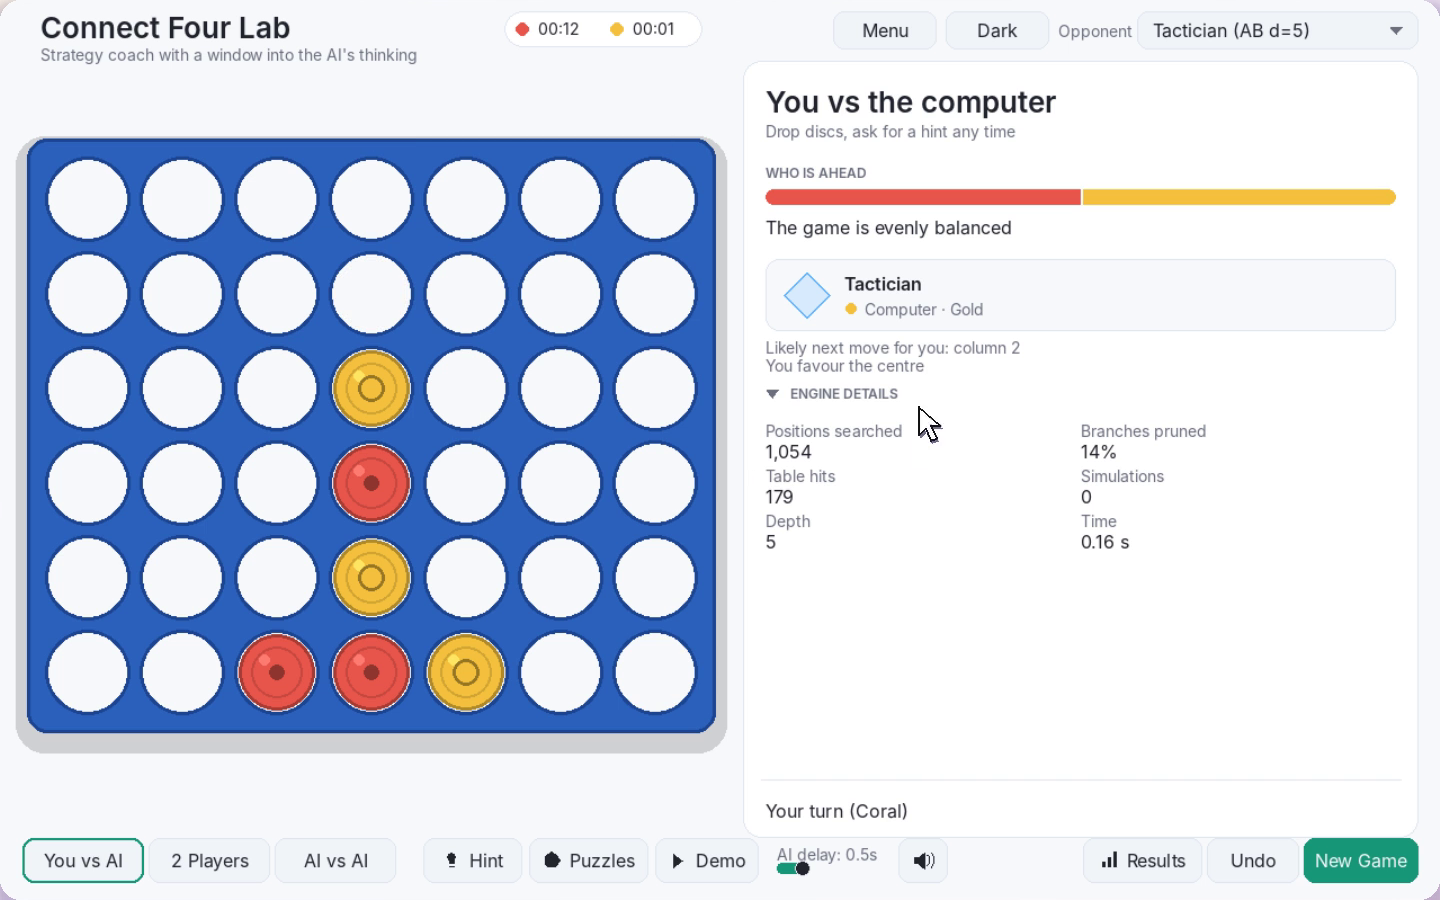
\includegraphics[width=\linewidth]{figures/app_engine.png}\caption{You vs AI with \emph{Engine details}: positions searched, branches pruned, table hits, depth and time, plus the predicted next move and playing style.}\end{subfigure}\hfill
\begin{subfigure}{0.49\textwidth}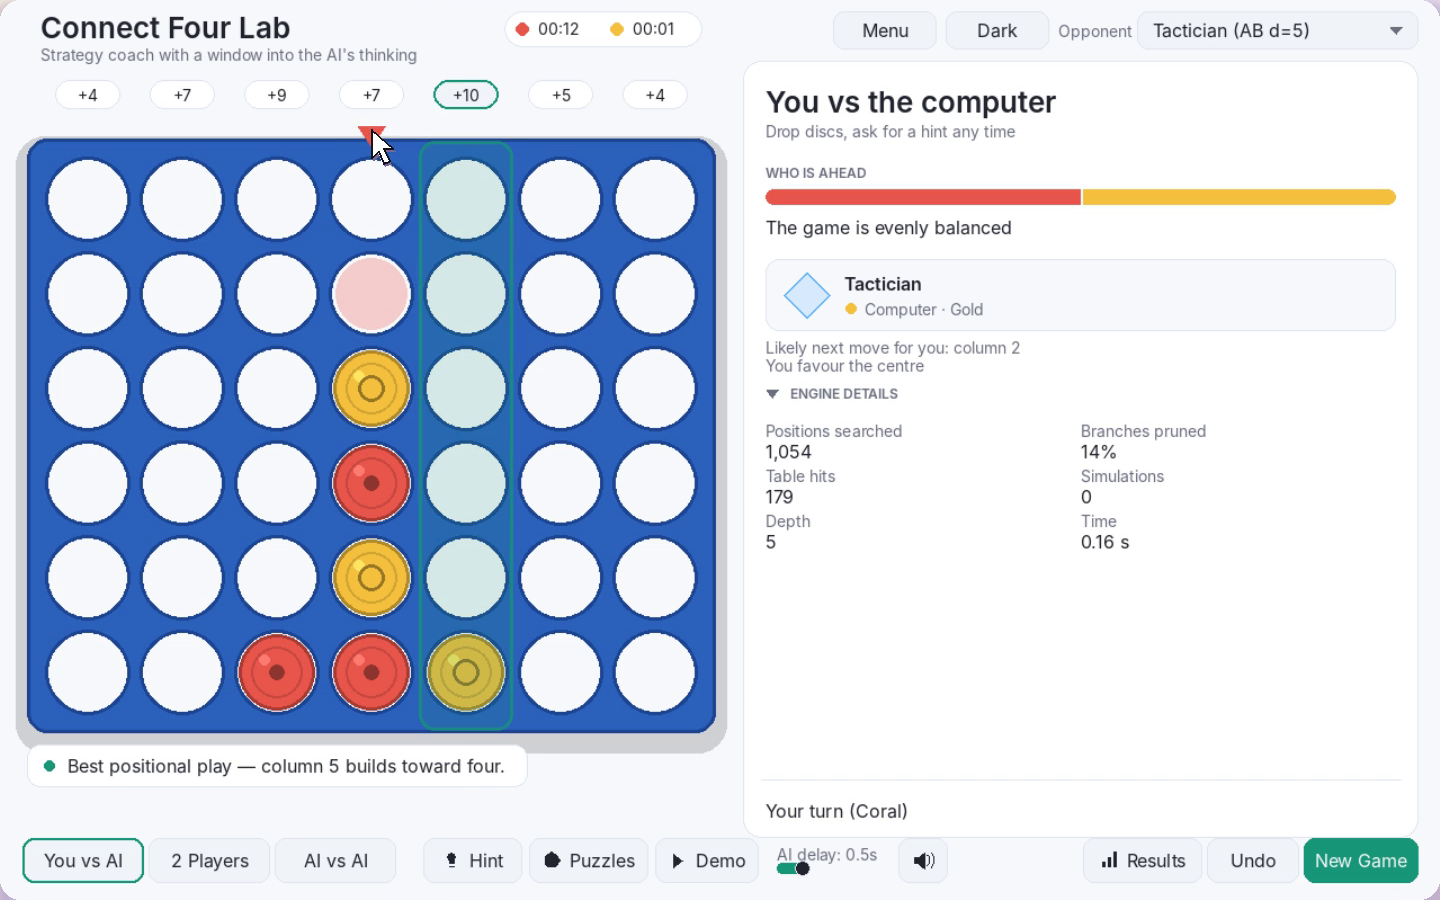
\includegraphics[width=\linewidth]{figures/app_hint.png}\caption{Hint: every column is scored by a depth-3 Alpha-Beta search (badges above the board) and the best move is explained in plain language.}\end{subfigure}\\[8pt]
\begin{subfigure}{0.49\textwidth}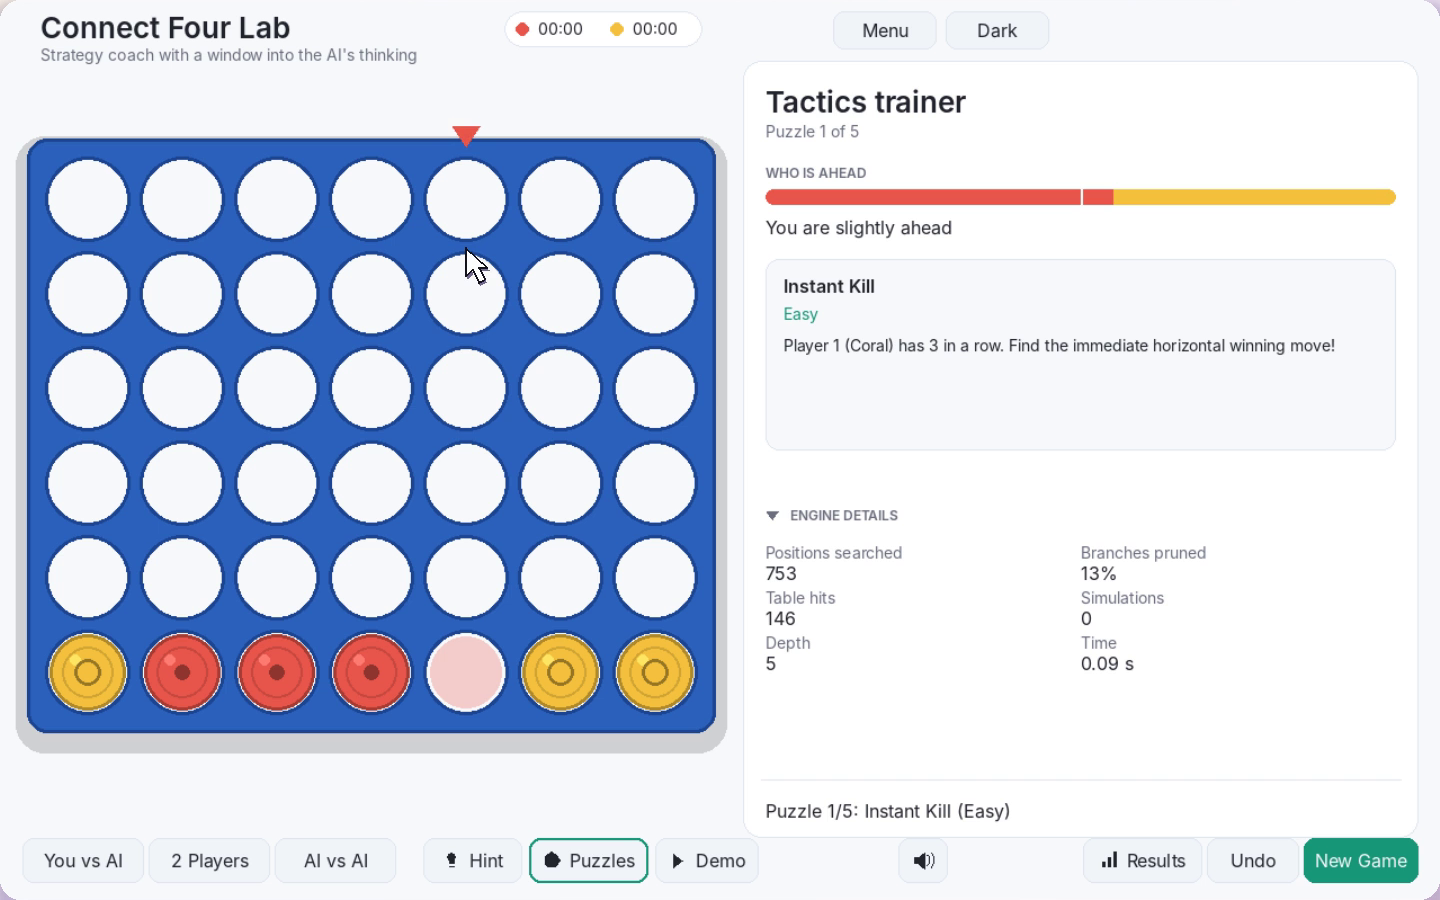
\includegraphics[width=\linewidth]{figures/app_puzzle.png}\caption{Tactics trainer: five puzzles from easy to hard, each with a description and an explanation once solved.}\end{subfigure}\hfill
\begin{subfigure}{0.49\textwidth}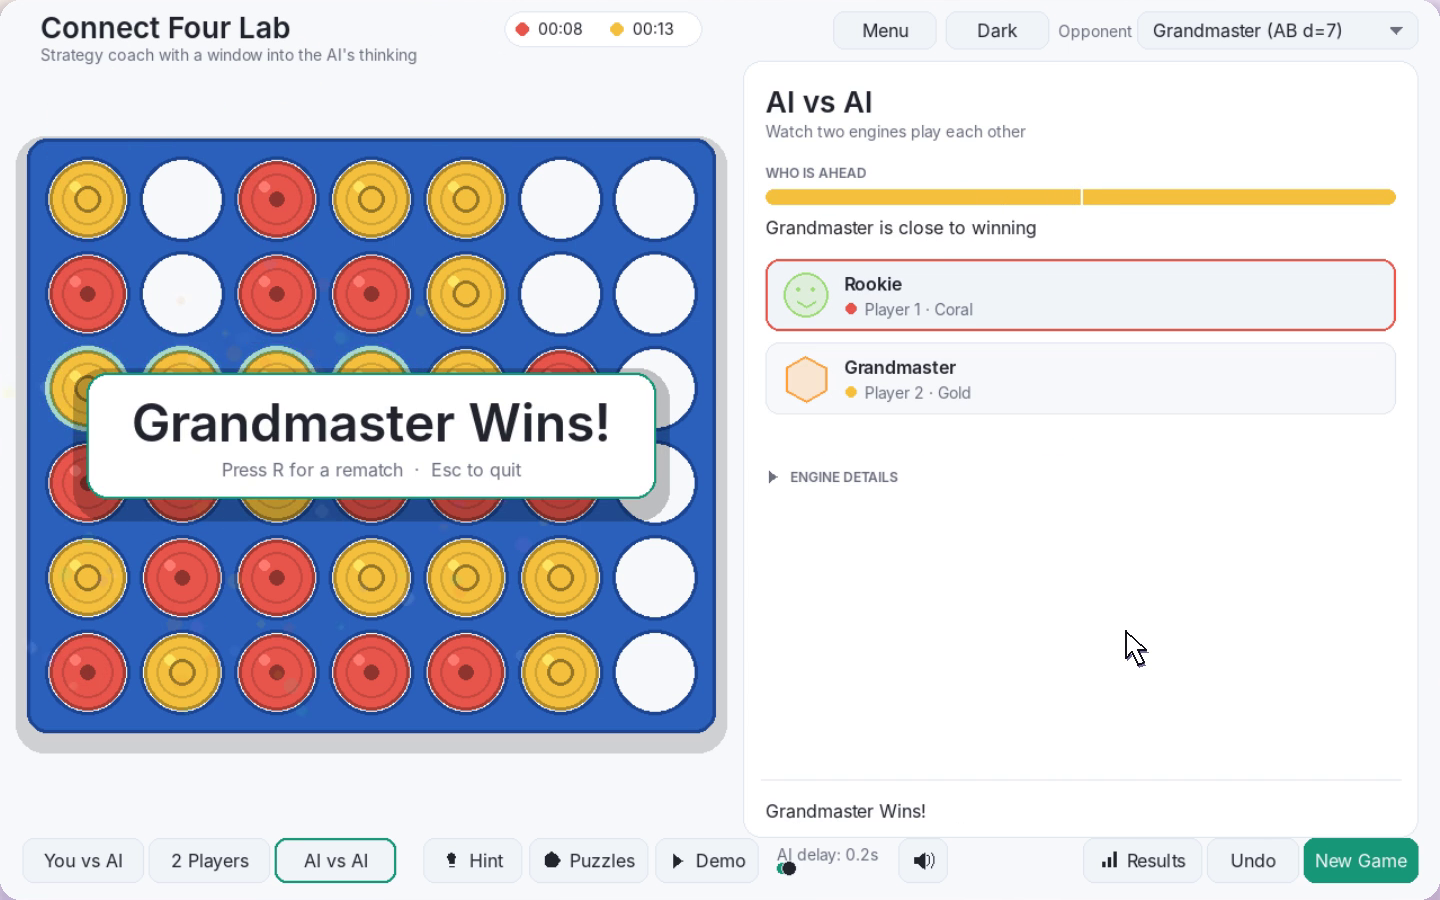
\includegraphics[width=\linewidth]{figures/app_avai.png}\caption{AI vs AI: Rookie (depth 2) against Grandmaster (iterative deepening to depth 7); the deeper engine wins.}\end{subfigure}
\caption{The strategy-coach application (screenshots from the recorded demo).}
\label{fig:app}
\end{figure}

\paragraph{Personas.} Four configured agents give a difficulty ladder (\cref{tab:personas}). All Alpha-Beta personas use the full evaluation weights and a transposition table.

\begin{table}[ht]
\centering\small
\caption{AI personas available in the application.}\label{tab:personas}
\begin{tabularx}{\textwidth}{@{}l l Y@{}}
\toprule
\textbf{Persona} & \textbf{Engine} & \textbf{Character} \\
\midrule
Rookie      & Alpha-Beta, depth 2, TT & Sees simple threats; instant replies. \\
Tactician   & Alpha-Beta, depth 5, TT & Solid tactical play, about 0.1\,s per move. \\
Grandmaster & Alpha-Beta, ID to depth 7, 1.5\,s limit, TT & Strongest; deepens as far as time allows. \\
Gambler     & MCTS, 1{,}000 simulations & Different style: judges moves by simulated games, not by evaluation. \\
\bottomrule
\end{tabularx}
\end{table}

\paragraph{Features.}
\begin{itemize}
  \item \textbf{Three modes:} You vs AI, two players and AI vs AI (with an adjustable delay between moves), plus a one-click demo.
  \item \textbf{Explanations:} a ``who is ahead'' bar ($\tanh$ of the evaluation, in words such as ``Tactician is clearly ahead''), hints with per-column scores and a one-line reason, a live ``best moves so far'' list while the AI is thinking, and the predicted next move and style.
  \item \textbf{Learning tools:} five tactics puzzles, an opening book that names the standard reply in the status line, undo, per-player clocks and adaptive difficulty that raises the opponent level after a winning streak.
  \item \textbf{Experiment results:} the four study charts can be browsed inside the app.
  \item \textbf{Presentation:} light and dark themes, drop and win animations, confetti and procedurally generated sound (no audio files).
\end{itemize}

\paragraph{Responsiveness.} The AI move and the hint search run in background threads, so the window never freezes, even during a 1.5\,s Grandmaster search. Each result is tagged with a \emph{generation number} that changes whenever a new game starts, the mode changes or the menu opens, and results from an older generation are discarded. Undo is disabled while the AI is thinking and cancels any pending hint. This prevents a slow search from playing a move into a game that no longer exists, a race condition that a dedicated test reproduces.

% =====================================================================
\section{Experimental Setup}\label{sec:setup}
% =====================================================================

\paragraph{Environment.} All experiments ran on a laptop with an Intel Core i7-12700H CPU under Linux, using Python~3.11.5 single-threaded, with no GPU. Raw results are written to \code{results/latest\_*.csv} by \code{python -m experiments.run\_all}, and the plots are drawn by \code{python -m experiments.plot\_results}.

\paragraph{Fair openings.} Alpha-Beta and Minimax are deterministic, so two agents starting from an empty board would replay the same game every time, and twenty games would contain only two distinct ones. Our first runs had exactly this flaw. In the final protocol, every \emph{pair} of games starts from its own seeded random 4-move opening (seed 42) and is played twice, once with each agent moving first. This gives varied but reproducible games and removes the first-move advantage.

\begin{table}[ht]
\centering\small
\caption{Settings of the four studies.}\label{tab:settings}
\begin{tabularx}{\textwidth}{@{}l Y c@{}}
\toprule
\textbf{Study} & \textbf{Configuration} & \textbf{Games} \\
\midrule
1. Ablation & Five depth-3 agents (Minimax, AB, AB+ordering, AB+ID with 1.0\,s, AB+TT) each vs Rookie (AB depth 2) & $5\times20$ \\
2. Tournament & Rookie (d2), Tactician (d5), Grandmaster (ID to d7, 2.0\,s), Gambler (MCTS, 500 sims); all six pairings & $6\times20$ \\
3. Depth vs time & Alpha-Beta depths 1--7 from the fixed position after moves 3\,3\,2\,4\,3\,2\,4\,2\,1\,5; mean of 5 runs & -- \\
4. Weight tuning & Default, aggressive and defensive weight sets at depth 3, each vs Tactician (d5) & $3\times60$ \\
\bottomrule
\end{tabularx}
\end{table}

All agents in all studies use the same full \code{WEIGHTS}, except where Study~4 deliberately changes them. The aggressive set doubles \code{three}, \code{playable\_three} and \code{center}. The defensive set doubles \code{double\_threat} and halves \code{center}; it also doubles \code{opp\_three}, which has no effect (\cref{tab:weights}).

% =====================================================================
\section{Results and Discussion}\label{sec:results}
% =====================================================================

\subsection{Study 1: Ablation, the cost of each optimisation}

\begin{figure}[ht]
\centering
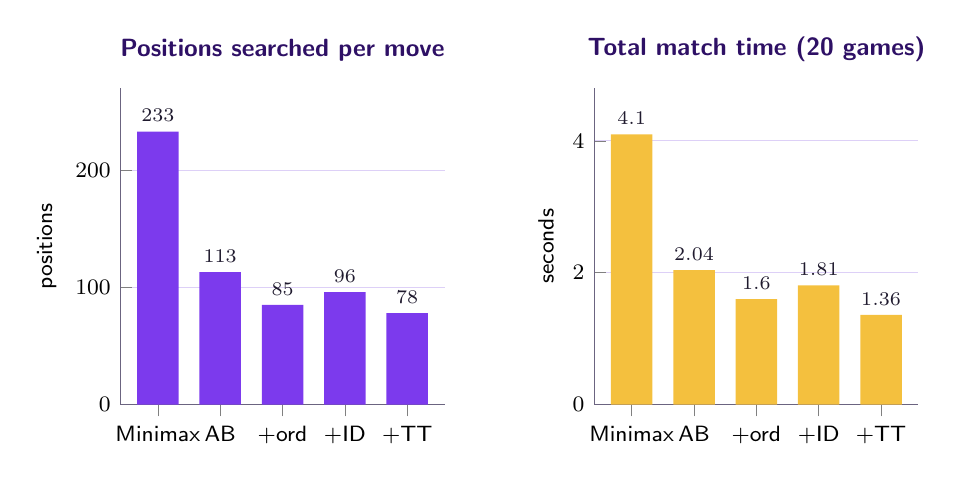
\begin{tikzpicture}
\begin{groupplot}[group style={group size=2 by 1,horizontal sep=1.9cm},
  width=0.47\textwidth,height=5.6cm,ybar,/pgf/bar width=15pt,ymin=0,
  symbolic x coords={Minimax,AB,+ord,+ID,+TT},xtick=data,
  axis line style={draw=muted},tick label style={font=\sffamily\footnotesize},
  label style={font=\sffamily\footnotesize},title style={font=\sffamily\small\bfseries,text=plum},
  ymajorgrids,grid style={draw=lavmid},nodes near coords,
  every node near coord/.append style={font=\sffamily\scriptsize,text=ink},
  enlarge x limits=0.15,axis x line*=bottom,axis y line*=left]
\nextgroupplot[title={Positions searched per move},ylabel={positions},ymax=270]
  \addplot[fill=violet,draw=none] coordinates {(Minimax,233) (AB,113) (+ord,85) (+ID,96) (+TT,78)};
\nextgroupplot[title={Total match time (20 games)},ylabel={seconds},ymax=4.8,
  every node near coord/.append style={/pgf/number format/.cd,fixed,precision=2}]
  \addplot[fill=gold,draw=none] coordinates {(Minimax,4.10) (AB,2.04) (+ord,1.60) (+ID,1.81) (+TT,1.36)};
\end{groupplot}
\end{tikzpicture}
\caption{Ablation at depth 3. Each bar adds one technique to Alpha-Beta (AB); \emph{+ID} and \emph{+TT} are each added on top of ordering.}
\label{fig:ablation}
\end{figure}

\begin{table}[ht]
\centering\small
\caption{Ablation results (20 games each vs Rookie). Win-rate 95\% confidence interval at $n=20$ is about $\pm22$ points.}\label{tab:ablation}
\begin{tabular}{@{}lccccc@{}}
\toprule
\textbf{Agent (depth 3)} & \textbf{Positions / move} & \textbf{Reduction} & \textbf{Wins / 20} & \textbf{Win rate} & \textbf{Match time} \\
\midrule
Minimax           & 233 & --    & 10 & 50\% & 4.10\,s \\
Alpha-Beta        & 113 & 52\%  & 10 & 50\% & 2.04\,s \\
+ move ordering   &  85 & 64\%  &  9 & 45\% & 1.60\,s \\
+ iterative deep. &  96 & 59\%  & 11 & 55\% & 1.81\,s \\
+ transp.\ table  & \textbf{78} & \textbf{67\%} &  9 & 45\% & \textbf{1.36\,s} \\
\bottomrule
\end{tabular}
\end{table}

\begin{keybox}[title=Finding 1]
At the same depth, the optimisations cut the search work by two thirds (233 $\to$ 78 positions per move) and the match time by the same proportion, while playing strength stays the same within statistical noise.
\end{keybox}

\textbf{Discussion.} Pruning alone halves the work. Ordering adds most of the remaining gain, because searching the centre first produces early cut-offs. Iterative deepening costs a little \emph{more} than ordering alone at a fixed depth (96 vs 85), because it searches depths 1 and 2 first. Its value is the time guarantee, not raw speed. The transposition table gives the lowest count by reusing transpositions. Win rates of 45--55\% are all inside the $\pm22$-point confidence interval: every row searches to the same depth, and Alpha-Beta is proven equal to Minimax, so equal strength is the \emph{expected} outcome. The small differences come from tie-breaking: when two moves score equally, a different search order can pick a different one, and the game then unfolds differently.

\subsection{Study 2: Tournament, strength of the personas}

\begin{table}[ht]
\centering\small
\caption{Head-to-head win rate of the \emph{row} agent against the \emph{column} agent (20 games per pairing). Remaining percentage points are losses and draws.}\label{tab:tournament}
\newcommand{\wc}[1]{\cellcolor{violet!\the\numexpr #1*7/10\relax}\ifnum#1>59 \color{white}\fi #1\%}
\begin{tabular}{@{}l|cccc|c@{}}
\toprule
\textbf{Row vs column} & \textbf{Rookie} & \textbf{Tactician} & \textbf{Grandmaster} & \textbf{Gambler} & \textbf{Total wins / 60} \\
\midrule
Rookie (AB d2)        & --      & \wc{15} & \wc{20} & \wc{45} & 16 \\
Tactician (AB d5)     & \wc{85} & --      & \wc{15} & \wc{85} & 37 \\
Grandmaster (ID d7)   & \wc{80} & \wc{80} & --      & \wc{70} & \textbf{46} \\
Gambler (MCTS 500)    & \wc{50} & \wc{15} & \wc{30} & --      & 19 \\
\bottomrule
\end{tabular}
\end{table}

\begin{keybox}[title=Finding 2]
Deeper search wins. The ranking follows search depth: Grandmaster (46 wins) $>$ Tactician (37) $>$ Gambler (19) $\approx$ Rookie (16).
\end{keybox}

\textbf{Discussion.} Grandmaster and Tactician each beat Rookie in 80--85\% of games, and Grandmaster beats Tactician 80\% of the time. MCTS with 500 random play-outs reaches only Rookie's level: it wins 50\% against Rookie but just 15\% against Tactician. Connect Four is highly tactical, and a random play-out often misses a forced sequence that a 5-ply Alpha-Beta search with a threat-aware evaluation sees directly. More simulations or smarter play-outs would strengthen MCTS (\cref{sec:future}). Grandmaster's matches took about ten times longer (107--119\,s against 10--20\,s), which is the price of the deeper search.

\subsection{Study 3: Depth versus time}

\begin{figure}[ht]
\centering
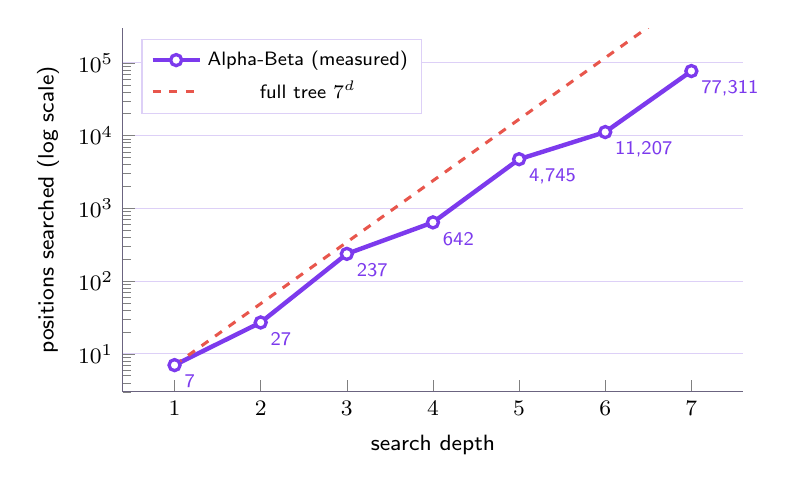
\begin{tikzpicture}
\begin{semilogyaxis}[width=0.78\textwidth,height=6.2cm,
  xlabel={search depth},ylabel={positions searched (log scale)},
  xtick={1,...,7},ymin=3,ymax=3e5,
  axis line style={draw=muted},tick label style={font=\sffamily\footnotesize},
  label style={font=\sffamily\footnotesize},
  ymajorgrids,grid style={draw=lavmid},legend style={font=\sffamily\scriptsize,draw=lavmid,at={(0.03,0.97)},anchor=north west},
  axis x line*=bottom,axis y line*=left]
  \addplot[violet,line width=1.6pt,mark=*,mark options={fill=white,line width=1.2pt},
     nodes near coords,point meta=explicit symbolic,every node near coord/.append style={font=\sffamily\scriptsize,anchor=north west,inner sep=3pt}]
    coordinates {(1,7)[7] (2,27)[27] (3,237)[237] (4,642)[642] (5,4745)[4{,}745] (6,11207)[11{,}207] (7,77311)[77{,}311]};
  \addlegendentry{Alpha-Beta (measured)}
  \addplot[coral,dashed,line width=1.1pt,domain=1:6.5,samples=12] {7^x};
  \addlegendentry{full tree $7^d$}
\end{semilogyaxis}
\end{tikzpicture}
\caption{Positions searched by Alpha-Beta at each depth, from one fixed mid-game position, compared with an unpruned tree.}
\label{fig:depth}
\end{figure}

\begin{table}[ht]
\centering\small
\caption{Depth study (Alpha-Beta with ordering, mean of 5 runs).}\label{tab:depth}
\begin{tabular}{@{}cccc@{}}
\toprule
\textbf{Depth} & \textbf{Positions} & \textbf{Time per move} & \textbf{Growth vs previous} \\
\midrule
1 & 7 & 0.0005\,s & -- \\
2 & 27 & 0.0017\,s & 3.9$\times$ \\
3 & 237 & 0.015\,s & 8.8$\times$ \\
4 & 642 & 0.035\,s & 2.7$\times$ \\
5 & 4{,}745 & 0.29\,s & 7.4$\times$ \\
6 & 11{,}207 & 0.57\,s & 2.4$\times$ \\
7 & 77{,}311 & 4.55\,s & 6.9$\times$ \\
\bottomrule
\end{tabular}
\end{table}

\begin{keybox}[title=Finding 3]
The effective branching factor, the geometric mean growth per level, is $(77{,}311/7)^{1/6} \approx \mathbf{4.7}$, against 7 for a full tree. At depth 7, Alpha-Beta searches 77 thousand positions instead of the $7^7 \approx 824$ thousand of an unpruned tree.
\end{keybox}

\textbf{Discussion.} Growth alternates between large steps (even $\to$ odd depth: $\times$6.9--8.8) and small ones (odd $\to$ even depth: $\times$2.4--3.9). This odd--even effect is characteristic of Alpha-Beta: the leaf count depends on whether the last ply belongs to the maximiser or the minimiser~\cite{knuth1975}. The timing explains our persona design. Depth~5 answers in about 0.3\,s and suits the Tactician. Depth~7 takes about 4.5\,s from this position, too slow for a fixed-depth opponent, which is why the Grandmaster uses iterative deepening with a 1.5\,s limit.

\subsection{Study 4: Evaluation weight tuning}

\begin{figure}[ht]
\centering
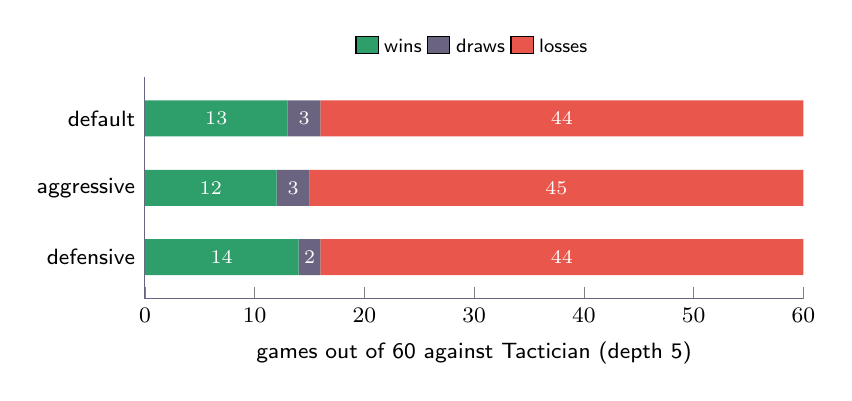
\begin{tikzpicture}
\begin{axis}[xbar stacked,width=0.82\textwidth,height=4.4cm,/pgf/bar width=13pt,
  xmin=0,xmax=60,xlabel={games out of 60 against Tactician (depth 5)},
  symbolic y coords={defensive,aggressive,default},ytick=data,
  axis line style={draw=muted},tick label style={font=\sffamily\footnotesize},label style={font=\sffamily\footnotesize},
  legend style={font=\sffamily\scriptsize,draw=none,at={(0.5,1.04)},anchor=south,legend columns=3},
  nodes near coords,every node near coord/.append style={font=\sffamily\scriptsize,text=white},
  enlarge y limits=0.3,axis x line*=bottom,axis y line*=left]
  \addplot[fill=good,draw=none] coordinates {(13,default) (12,aggressive) (14,defensive)};
  \addplot[fill=muted,draw=none] coordinates {(3,default) (3,aggressive) (2,defensive)};
  \addplot[fill=coral,draw=none] coordinates {(44,default) (45,aggressive) (44,defensive)};
  \legend{wins,draws,losses}
\end{axis}
\end{tikzpicture}
\caption{Results of three evaluation weight sets at depth 3 against a depth-5 opponent (60 games each).}
\label{fig:weights}
\end{figure}

\begin{keybox}[title=Finding 4]
The three weight sets score 13, 12 and 14 wins out of 60, a spread of 3.3 percentage points against a 95\% confidence interval of about $\pm$10 points. \textbf{At a fixed depth, these weight changes make no measurable difference; search depth matters far more.}
\end{keybox}

\textbf{Discussion.} An earlier 20-game run suggested that the defensive set was best (6 vs 4 vs 3 wins). We did not report that as a result. We tripled the sample to 60 games, and the gap disappeared, showing that the first ``winner'' was chance. This is the most important methodological lesson of the project: small samples produce convincing-looking but false conclusions. Against an opponent searching two plies deeper, all three variants lose about three games in four, which agrees with Study~2: depth dominates evaluation tuning.

% =====================================================================
\section{Testing and Verification}\label{sec:testing}
% =====================================================================

Testing was part of every layer, not an afterthought. The suite contains \textbf{209 tests} and runs in about 15 seconds:

\begin{center}
\begin{tcolorbox}[enhanced,colback=ink,colframe=ink,arc=3pt,width=0.62\textwidth,left=10pt,boxrule=0pt]
\color{white}\ttfamily\small \$ python -m pytest -q\\
\color{good!60!white}209 passed\color{white} in 14.01s
\end{tcolorbox}
\end{center}

\begin{table}[ht]
\centering\small
\caption{Test suite by area. Several tests check \emph{invariants} rather than examples.}\label{tab:tests}
\begin{tabularx}{\textwidth}{@{}l c Y@{}}
\toprule
\textbf{Test file} & \textbf{Tests} & \textbf{What is verified} \\
\midrule
\code{test\_board} & 19 & gravity, full columns, all win directions, undo, hashing; local win check equals full scan over 1{,}000 random games \\
\code{test\_agents} & 9 & Random/Greedy/Minimax behaviour; Minimax d3 beats Random $\ge$18/20; finds a forced win \\
\code{test\_alphabeta} & 2 & \textbf{same move and score as Minimax} on 50 seeded positions, depths 1--4; fewer nodes at depth 5 \\
\code{test\_alphabeta\_iterative} & 4 & ordering never changes scores; time limit respected (0.2\,s limit answered within 0.3\,s) \\
\code{test\_zobrist} & 7 & incremental hash equals recomputed hash; \textbf{TT never changes the root score}; bounded size \\
\code{test\_evaluation} & 110 & \textbf{symmetry} $\text{eval}(s,1)=-\text{eval}(s,2)$ on 100 positions; full weights beat basic weights \\
\code{test\_mcts} & 7 & beats Random $\ge$19/20; takes wins; blocks losses; same seed gives same move \\
\code{test\_predictor} & 7 & win/block priority, full board, style thresholds, board restored \\
\code{test\_gui}, \code{test\_hint}, \code{test\_puzzles} & 31 & widgets, animations, stale-result gate, hint scores, every puzzle solvable \\
\code{test\_arena}, \code{test\_report}, \code{test\_setup} & 13 & fair openings, CSV output, report generation, environment checks \\
\midrule
\textbf{Total} & \textbf{209} & \\
\bottomrule
\end{tabularx}
\end{table}

Two safeguards keep the documentation honest. The report generator (\code{python -m report.generate}) first runs the full test suite and refuses to write the report if any test fails. All tables in the generated report are built directly from the CSV files, so the numbers in the documentation always match the latest experiment run.

% =====================================================================
\section{Limitations}\label{sec:limits}
% =====================================================================

\begin{itemize}
  \item \textbf{Not perfect play.} The agents search to a limited depth with a heuristic evaluation. Connect Four is solved~\cite{allis1988}, but we do not use a solver or an endgame database, so a perfect player can still beat Grandmaster.
  \item \textbf{Python speed.} The board is a list of lists and the evaluation re-scans all 69 windows at every leaf. A bitboard engine would be one to two orders of magnitude faster and could search several plies deeper in the same time.
  \item \textbf{Simple MCTS.} Play-outs are random and the tree is rebuilt for every move instead of reusing the subtree, which explains MCTS's modest strength in Study~2.
  \item \textbf{Hand-set weights.} The evaluation weights were chosen by hand and compared in only three variants. Two keys in the dictionary (\code{opp\_two}, \code{opp\_three}) are unused because of the symmetric design.
  \item \textbf{Shallow player model.} The predictor assumes a one-move-ahead opponent and the style description uses fixed thresholds; it informs the player but does not influence the AI's move choice.
  \item \textbf{Transposition table.} There is no verification against the rare hash collision and no ageing; once the table is full, new positions are simply not stored.
  \item \textbf{Statistical power.} Twenty games per pairing gives confidence intervals of about $\pm$22 points, enough to rank agents of clearly different strength but not to separate close ones.
  \item \textbf{Minor interface issues.} With \emph{Engine details} open in AI vs AI mode, the statistics of both engines overflow the panel, and a puzzle that has two winning moves accepts only one.
\end{itemize}

% =====================================================================
\section{Future Work}\label{sec:future}
% =====================================================================

\begin{enumerate}
  \item \textbf{Bitboards and incremental evaluation} to make search much faster, and therefore deeper at the same time limit.
  \item \textbf{Stronger move ordering} with killer-move and history heuristics, and principal-variation search.
  \item \textbf{Better MCTS:} tree reuse between moves, ``light'' or heavy play-outs by default, and an Alpha-Beta/MCTS hybrid.
  \item \textbf{Automatic weight tuning} through self-play (for example, a simple evolutionary strategy), with larger matches and reported confidence intervals.
  \item \textbf{Use the opponent model} to bias the search towards the human's likely replies, and let the AI use the opening book for its own moves.
  \item \textbf{An endgame solver} that switches to exact search when few empty cells remain.
\end{enumerate}

% =====================================================================
\section{Conclusion}\label{sec:conclusion}
% =====================================================================

We built a Connect Four AI that meets every part of the brief. It \emph{evaluates possible moves} with a threat-aware heuristic over 69 windows, \emph{predicts the player's strategy} both inside the Minimax search and visibly through an explicit player model, and \emph{chooses optimal plays} within its search horizon using Alpha-Beta pruning. Beyond the brief, we added a second AI paradigm (MCTS), a coaching application that explains the AI's reasoning, four reproducible experiments and 209 automated tests.

The measurements give a clear picture. Alpha-Beta's optimisations remove two thirds of the search work without changing a single decision. Search depth is the main driver of playing strength. Evaluation weight changes matter far less than depth. And a 20-game sample can show a false winner that disappears at 60 games. The last lesson extends beyond games: claims should be measured, and measurements should be large enough to trust.

% =====================================================================
\section*{Team and Contributions}
\addcontentsline{toc}{section}{Team and Contributions}
% =====================================================================

\begin{center}
\small
\begin{tabularx}{\textwidth}{@{}l Y Y@{}}
\toprule
\textbf{Member} & \textbf{Area of responsibility} & \textbf{Main files} \\
\midrule
Satyam Singh & Problem definition, game engine and baseline agents (Random, Greedy) & \code{game/board.py}, \code{agents/simple.py} \\
Shivam Chaurasia & Agent interface, evaluation function, Minimax, application and live demo & \code{agents/base.py}, \code{agents/evaluation.py}, \code{agents/minimax.py}, \code{gui/} \\
Manish Shroyan & Alpha-Beta pruning, move ordering, Monte Carlo Tree Search; test suite & \code{agents/alphabeta.py}, \code{agents/mcts.py}, \code{tests/} \\
Mitu Kumar & Iterative deepening, transposition table and Zobrist hashing, player predictor, experiments, results analysis and report & \code{agents/alphabeta.py} (iterative deepening), \code{agents/zobrist.py}, \code{agents/predictor.py}, \code{experiments/}, \code{report/} \\
\bottomrule
\end{tabularx}
\end{center}

% =====================================================================
\begin{thebibliography}{99}
\addcontentsline{toc}{section}{References}
\small
\bibitem{aima} S.~Russell and P.~Norvig, \emph{Artificial Intelligence: A Modern Approach}, 4th ed. Pearson, 2020, ch.~5 (Adversarial Search and Games).
\bibitem{shannon1950} C.~E.~Shannon, ``Programming a computer for playing chess,'' \emph{Philosophical Magazine}, vol.~41, no.~314, pp.~256--275, 1950.
\bibitem{knuth1975} D.~E.~Knuth and R.~W.~Moore, ``An analysis of alpha-beta pruning,'' \emph{Artificial Intelligence}, vol.~6, no.~4, pp.~293--326, 1975.
\bibitem{korf1985} R.~E.~Korf, ``Depth-first iterative-deepening: An optimal admissible tree search,'' \emph{Artificial Intelligence}, vol.~27, no.~1, pp.~97--109, 1985.
\bibitem{zobrist1970} A.~L.~Zobrist, ``A new hashing method with application for game playing,'' Technical Report~88, Computer Sciences Department, University of Wisconsin, 1970.
\bibitem{kocsis2006} L.~Kocsis and C.~Szepesv\'ari, ``Bandit based Monte-Carlo planning,'' in \emph{Proc.\ European Conference on Machine Learning (ECML)}, 2006, pp.~282--293.
\bibitem{auer2002} P.~Auer, N.~Cesa-Bianchi and P.~Fischer, ``Finite-time analysis of the multiarmed bandit problem,'' \emph{Machine Learning}, vol.~47, pp.~235--256, 2002.
\bibitem{browne2012} C.~B.~Browne \emph{et al.}, ``A survey of Monte Carlo tree search methods,'' \emph{IEEE Trans.\ Computational Intelligence and AI in Games}, vol.~4, no.~1, pp.~1--43, 2012.
\bibitem{allis1988} L.~V.~Allis, ``A knowledge-based approach of Connect-Four: The game is solved: White wins,'' M.Sc.\ thesis, Vrije Universiteit Amsterdam, 1988.
\bibitem{edelkamp2008} S.~Edelkamp and P.~Kissmann, ``Symbolic classification of general two-player games,'' in \emph{KI 2008: Advances in Artificial Intelligence}, LNCS~5243, Springer, 2008, pp.~185--192.
\bibitem{pygame} Pygame Community, \emph{Pygame 2.6 documentation}, \url{https://www.pygame.org/docs/}.
\end{thebibliography}

% =====================================================================
\appendix
\section{Running the Project}\label{app:run}
% =====================================================================

\begin{tcolorbox}[enhanced,colback=lavender!40,colframe=lavmid,boxrule=0.5pt,arc=3pt,left=8pt]
\ttfamily\small
git clone \repourl.git\\
cd Four-in-a-row-2\\
python -m venv .venv \&\& source .venv/bin/activate\\
pip install -r requirements.txt\\[4pt]
python -m gui.app \hfill\color{muted}\# play the game\color{ink}\\
python -m pytest \hfill\color{muted}\# run all 209 tests\color{ink}\\
python -m experiments.run\_all -{}-quick \hfill\color{muted}\# smoke run of the 4 studies\color{ink}\\
python -m experiments.run\_all \hfill\color{muted}\# full run (about 8 minutes)\color{ink}\\
python -m experiments.plot\_results \hfill\color{muted}\# draw the figures\color{ink}\\
python -m report.generate \hfill\color{muted}\# test, then build the results report
\end{tcolorbox}

\section{Repository Structure}

\begin{center}
\small
\begin{tabularx}{\textwidth}{@{}l Y@{}}
\toprule
\textbf{Path} & \textbf{Contents} \\
\midrule
\code{config.py} & all constants: board size, win score, move order, table size, seeds, UCB constant \\
\code{game/board.py} & board, rules, win detection, undo, incremental Zobrist hash \\
\code{agents/} & \code{base} (interface, statistics), \code{simple}, \code{minimax}, \code{alphabeta}, \code{zobrist}, \code{evaluation}, \code{mcts}, \code{predictor} \\
\code{gui/} & \code{app} (main loop, threads), \code{board\_view}, \code{panel}, \code{hint}, \code{puzzles}, \code{opening\_book}, \code{animation}, \code{sound}, \code{screens}, \code{widgets}, \code{theme} \\
\code{experiments/} & \code{arena} (match runner, fair openings), \code{run\_all} (four studies), \code{plot\_results} \\
\code{report/} & report generator and generated Markdown/HTML report \\
\code{results/} & CSV outputs and figures of the latest experiment run \\
\code{tests/} & 209 tests, one file per layer, with shared helpers \\
\bottomrule
\end{tabularx}
\end{center}

In total the project contains about 3{,}000 lines of application code and 1{,}400 lines of tests.

\end{document}
